\documentclass[reprint, amsmath, amssymb, aps, pra, nofootinbib]{revtex4-2}


% --- Основные пакеты ---
\usepackage[T2A]{fontenc}
\usepackage[utf8]{inputenc}
\usepackage[russian,english]{babel}

\usepackage{graphicx}
\usepackage{bm}
\usepackage{float}
\usepackage{subcaption} 

% Настройка гиперссылок
\usepackage[unicode, colorlinks=true, linkcolor=blue, citecolor=blue, urlcolor=blue]{hyperref}

\begin{document}

\title{Опыт Милликена (Лабораторная работа 3.3.3)}

% --- Авторы ---
\author{Иван Рудко}
\email{rudko.ia@phystech.edu} 
\affiliation{Московский физико-технический университет, группа Б02-506}

\author{Ефим Сычев}
\email{sychev.ea@phystech.edu}
\affiliation{Московский физико-технический университет, группа Б02-506}

\date{\today}

\begin{abstract}
В данной работе описываются физические принципы и экспериментальная база для измерения элементарного электрического заряда методом масляных капель (опыт Милликена). Рассмотрены уравнения движения заряженной капли в вязкой среде при наличии и отсутствии внешнего электрического поля. Классическая методика визуального наблюдения заменена на автоматизированный программный трекинг капель масла на видеозаписи, что позволило вычислять заряд капель на основе статистического анализа их установившихся скоростей. Экспериментально полученное значение элементарного заряда составило $(1.594 \pm 1.034) \cdot 10^{-19}$ Кл, что отклоняется от справочного значения лишь на $1.6\%$.
\end{abstract}

\maketitle

% --- Основной текст ---
\section{ВВЕДЕНИЕ}
Основной целью данной работы является измерение элементарного электрического заряда методом масляных капель с использованием автоматизированного компьютерного анализа видеотреков.

Если элементарный заряд действительно существует, то заряд $q$ любого тела может принимать только дискретную последовательность значений:
\begin{equation}
    q = 0, \pm e, \pm 2e, \pm 3e, \dots \pm ne, \dots,
    \label{eq:discreteness}
\end{equation}
где $e$ — элементарный заряд. В предлагаемом опыте измеряется заряд небольших капелек масла, несущих всего несколько избыточных электронов. Сравнивая между собой заряды капель, можно убедиться, что все они по модулю кратны одной и той же фундаментальной величине $e$.

Экспериментальная установка включает в себя плоский конденсатор в защитном кожухе, осветитель и пульверизатор с маслом. Для управления полем используется электростатический вольтметр с переключателем напряжения, а наблюдение за рабочим объемом ведется через измерительный микроскоп, оснащенный цифровой видеокамерой.

\section{ФИЗИЧЕСКИЕ ОСНОВЫ ЯВЛЕНИЯ}
В отличие от классической методики, где измеряются времена прохождения фиксированного расстояния, в данной работе применяется компьютерный трекинг частиц. Это позволяет извлекать из видеозаписей мгновенные координаты капель и непрерывно вычислять их установившиеся скорости.

\subsection{Определение радиуса капли}
При свободном падении капли в воздухе (электрическое поле выключено) достигается установившаяся скорость падения $v_{\text{пад}}$, при которой сила тяжести уравновешивается силой вязкого трения Стокса:
\begin{equation}
    mg = F_{\text{тр}} \implies \frac{4}{3}\pi r^3 \rho g = 6\pi\eta r v_{\text{пад}},
\end{equation}
где $r$ — радиус капли, $\eta$ — динамическая вязкость воздуха, $\rho$ — плотность масла, $g$ — ускорение свободного падения. Из этого условия однозначно определяется радиус капли:
\begin{equation}
    r = \sqrt{\frac{9\eta v_{\text{пад}}}{2\rho g}}.
    \label{eq:radius}
\end{equation}

\subsection{Определение заряда капли}
При включении электрического поля плоского конденсатора капля с зарядом $q$ начинает двигаться вверх. Напряжённость поля равна $E = U/l$, где $l$ — расстояние между пластинами, $U$ — разность потенциалов. 

При установившемся движении вверх со скоростью $v_{\text{под}}$ электрическая сила преодолевает силу тяжести и силу сопротивления воздуха:
\begin{equation}
    qE = mg + F_{\text{тр}} \implies q\frac{U}{l} = \frac{4}{3}\pi r^3 \rho g + 6\pi\eta r v_{\text{под}}.
\end{equation}
Отсюда получается итоговая расчётная формула для заряда капли:
\begin{equation}
    q = \frac{l}{U} \left( 6\pi\eta r v_{\text{под}} + \frac{4}{3}\pi r^3 \rho g \right).
    \label{eq:charge_final}
\end{equation}
Деление вычисленного заряда $q$ на справочное значение элементарного заряда $e$ позволяет найти число избыточных электронов $n$ на исследуемой капле.

\section{ЭКСПЕРИМЕНТАЛЬНАЯ УСТАНОВКА}
Схема установки представлена на рис. \ref{fig:setup}. Масло разбрызгивается пульверизатором и попадает в плоский конденсатор $C$ через отверстие в верхней пластине. Напряжение на пластины подаётся от выпрямителя и измеряется вольтметром $V$. Ключ $K$ позволяет менять направление электрического поля.

\begin{figure}[ht]
    \centering
    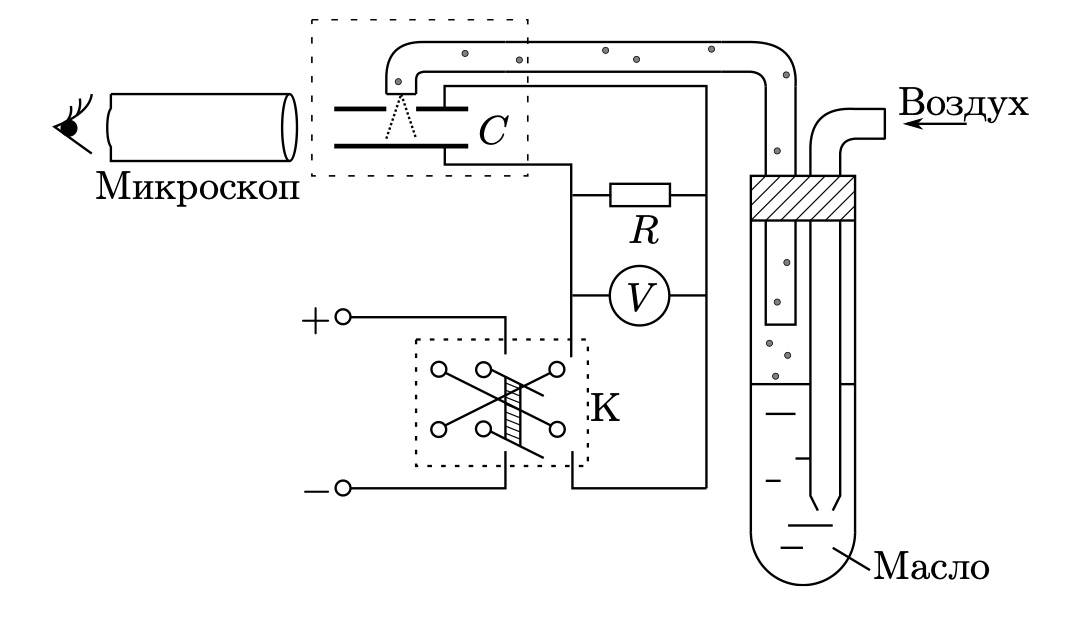
\includegraphics[width=0.9\linewidth]{stage.jpeg} 
    \caption{Схема экспериментальной установки.}
    \label{fig:setup}
\end{figure}

Главным отличием от визуальной методики является способ регистрации данных. Измерительный микроскоп снабжен цифровой видеокамерой, передающей изображение на ПК, благодаря чему процесс движения капель записывается в формате видеофайла с фиксированной частотой 50 кадров/с.

\section{ХОД РАБОТЫ И ПРОГРАММНАЯ ОБРАБОТКА}

\subsection{Проведение эксперимента и видеофиксация}
Для наблюдения использовался метод тёмного поля: свет от осветителя направлялся под углом к оси микроскопа, из-за чего капли масла рассеивали свет и выглядели как светящиеся точки на черном фоне (рис. \ref{fig:frame}).

С помощью пульверизатора в рабочее пространство конденсатора впрыскивалось облачко капель. В течение первых 5–10 секунд электрическое поле оставалось выключенным для оседания наиболее крупных частиц. Затем на пластины подавалось рабочее напряжение $U = 230$~В и начиналась запись. В процессе съёмки периодически замыкался и размыкался ключ $K$, заставляя группы капель падать под действием силы тяжести и подниматься в электрическом поле. Для обеспечения достаточной статистической выборки было записано 10 видеофайлов.

\begin{figure}[h]
    \centering
    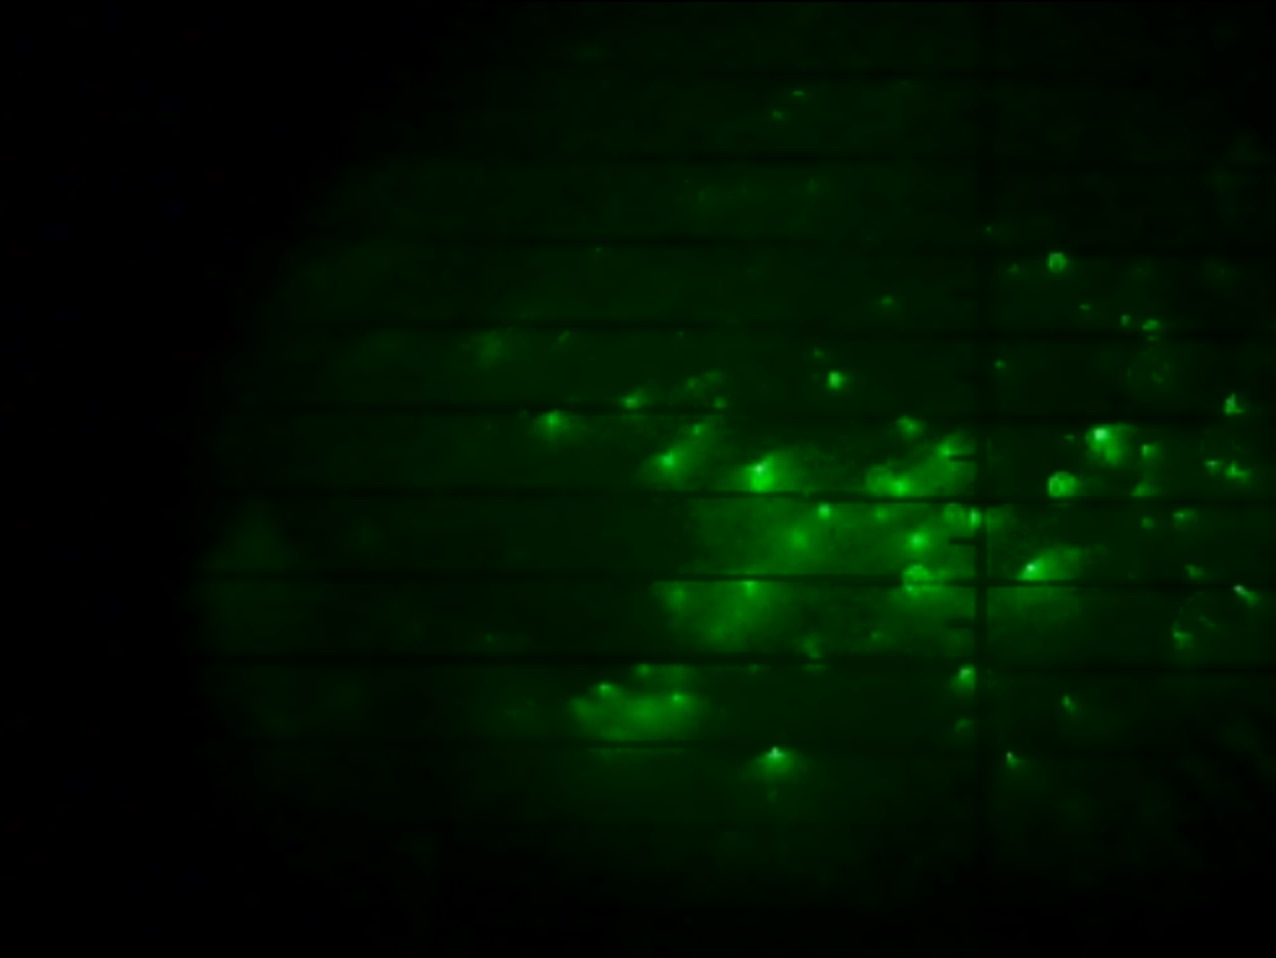
\includegraphics[width=0.9\linewidth]{screenshot1.jpeg}
    \caption{Необработанный кадр из видеофайла (изображение в тёмном поле).}
    \label{fig:frame}
\end{figure}

\subsection{Программная обработка данных}
Для извлечения физических величин был разработан скрипт на языке Python с использованием библиотек \texttt{OpenCV}, \texttt{trackpy} и \texttt{SciPy}. 

На первом этапе алгоритм осуществляет покадровый трекинг: детектирует светящиеся капли по порогу яркости и массе, после чего связывает их в непрерывные траектории $y(t)$. Затем проводится анализ кинематики. Чтобы подавить пиксельный шум, к координатам применяется фильтр Савицкого-Голея, а мгновенная скорость вычисляется как градиент координаты. Программа автоматически разбивает траектории на интервалы падения ($v > 0$) и подъема ($v < 0$). Наконец, для стабильных участков находятся медианные скорости $v_{\text{пад}}$ и $v_{\text{под}}$, что позволяет по формулам \eqref{eq:radius} и \eqref{eq:charge_final} определить радиус и полный заряд $q$ каждой отдельной капли.

Результаты автоматизированной обработки (траектории, распределения скоростей и уровни зарядов) для одной из серий приведены на рис. \ref{fig:triangle_plots}. Графики для остальных видеофайлов вынесены в Приложение А.

\begin{figure*}[ht]
    \centering
    \begin{subfigure}[b]{0.45\textwidth}
        \centering
        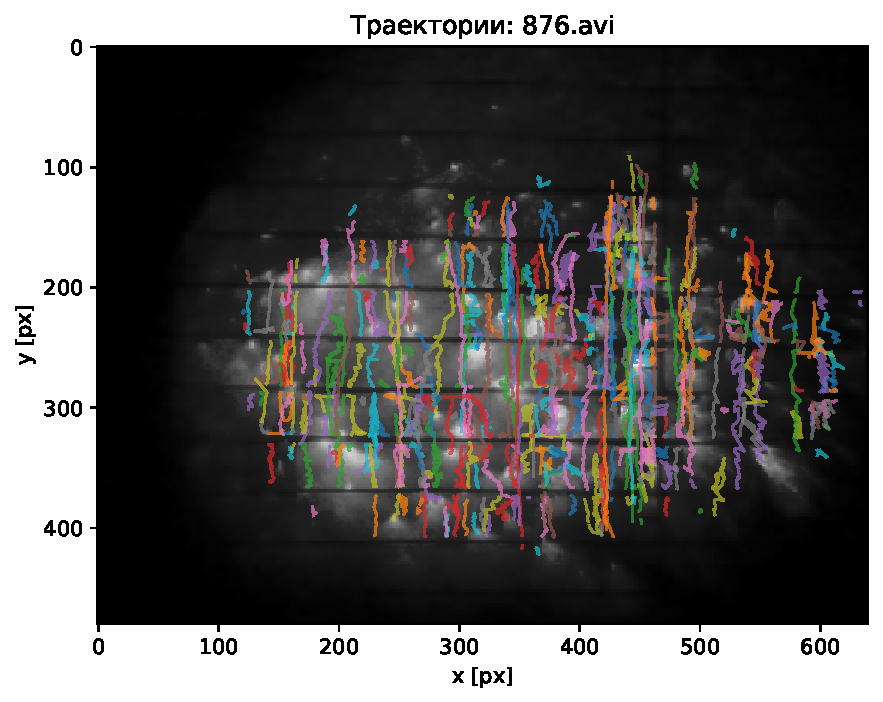
\includegraphics[width=\textwidth]{876_1_trajectories.pdf}
        \caption{Траектории капель}
        \label{fig:traj_main}
    \end{subfigure}
    \vspace{1em}
    
    \begin{subfigure}[b]{0.45\textwidth}
        \centering
        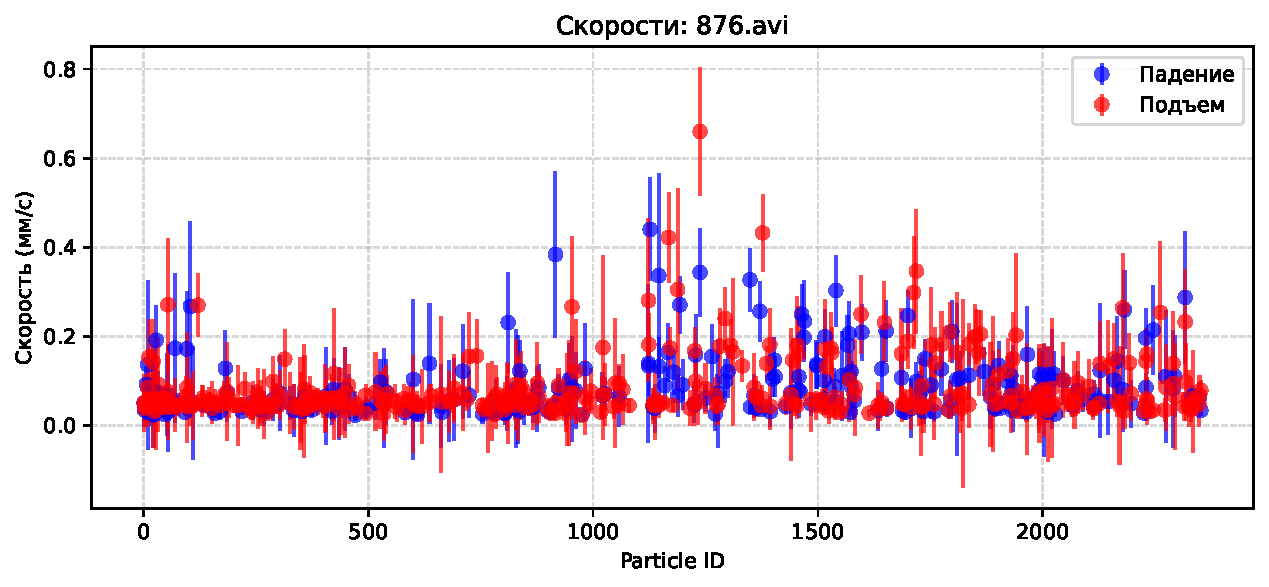
\includegraphics[width=\textwidth]{876_2_speeds.pdf}
        \caption{Мгновенные скорости}
        \label{fig:speeds_main}
    \end{subfigure}
    \hfill 
    \begin{subfigure}[b]{0.45\textwidth}
        \centering
        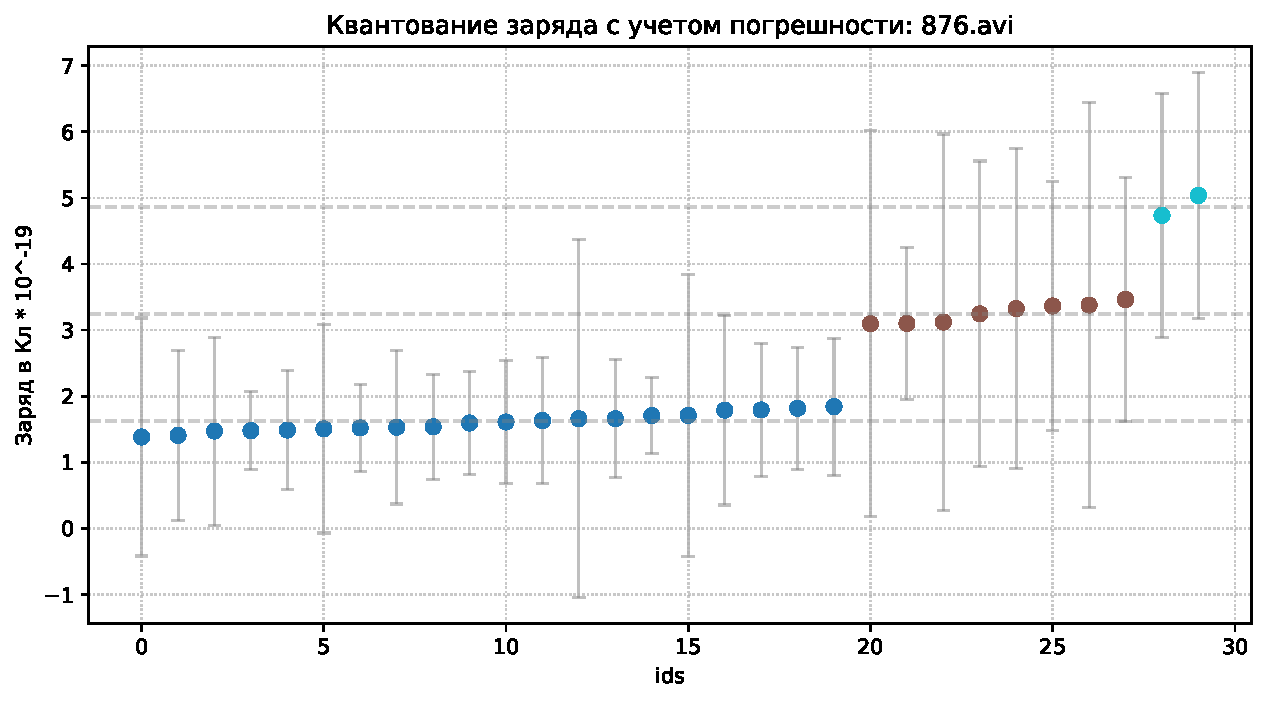
\includegraphics[width=\textwidth]{876_3_quantization.pdf}
        \caption{Дискретность заряда}
        \label{fig:quant_main}
    \end{subfigure}
    \caption{Поэтапная обработка видеофайла \texttt{876} алгоритмом компьютерного зрения. Видно извлечение траекторий (а), фильтрацию скоростей с расчетом погрешностей (б) и квантование уровней заряда (в).}
    \label{fig:triangle_plots}
\end{figure*}

\section{ОЦЕНКА ПОГРЕШНОСТЕЙ}
В классическом визуальном методе основным фактором ошибки выступает время реакции экспериментатора. Переход к программной покадровой обработке снижает погрешность определения времени одного кадра до $0.02$ с. 

Тем не менее, предложенный метод имеет свои специфические источники ошибок. Во-первых, это пиксельный шум при определении центроид капель, который формирует инструментальную межкадровую дисперсию. Во-вторых, неизбежны неточности пространственной калибровки масштаба. Кроме того, во время наблюдения происходит испарение масляных капель, из-за чего их радиус $r$ может меняться прямо в процессе измерения. Для минимизации влияния случайных межкадровых флуктуаций в алгоритме применялось усреднение по медиане на длительных непрерывных участках.

\section{РЕЗУЛЬТАТЫ ЭКСПЕРИМЕНТА}

Анализ 10 видеофайлов позволил собрать статистику для 107 валидных капель. Объединённое распределение зарядов со всех серий измерений представлено на рис. \ref{fig:final_dist}.

\begin{figure*}[ht]
    \centering
    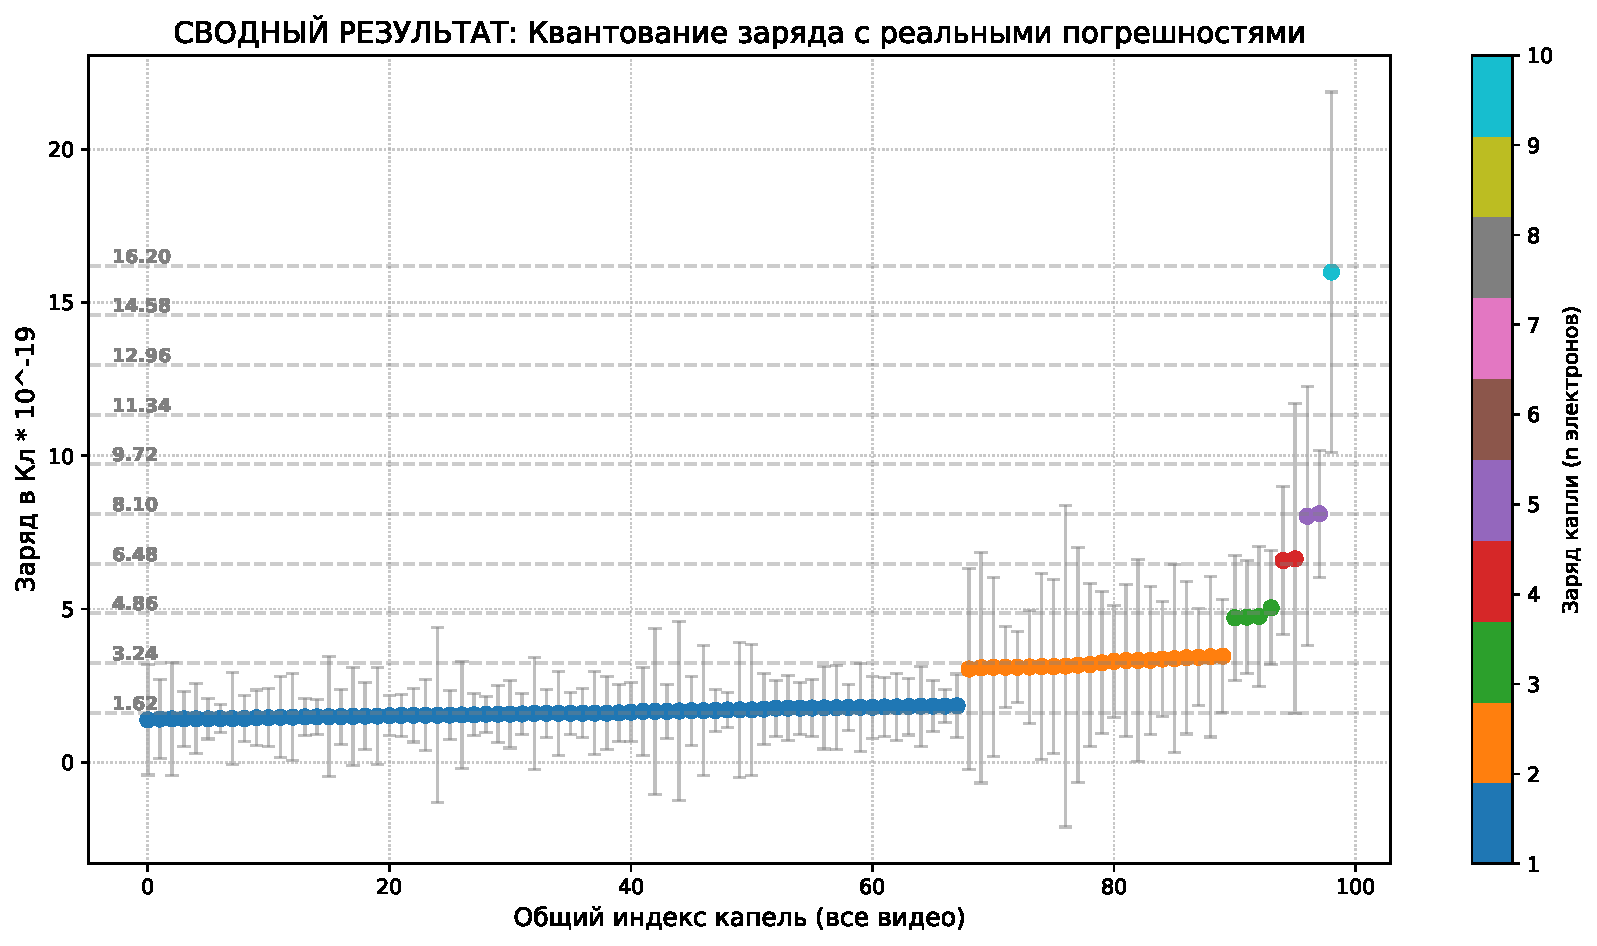
\includegraphics[width=0.8\textwidth]{Milliken/FINAL_SUMMARY_quantization.pdf}
    \caption{Итоговое распределение зарядов капель (сводный график по 107 каплям).}
    \label{fig:final_dist}
\end{figure*}

Экспериментально полученное значение элементарного заряда в системе СИ составило $e_{\text{эксп}} = (1.594 \pm 1.034) \cdot 10^{-19}$ Кл (при справочном значении $1.620 \cdot 10^{-19}$ Кл). В системе СГС этот результат соответствует $(4.779 \pm 3.100) \cdot 10^{-10}$ ед. СГС против табличных $4.857 \cdot 10^{-10}$ ед. СГС.

Отклонение полученного медианного результата от табличной константы составило 1.6\%, что говорит о высокой точности самого эксперимента. При этом формальная полная погрешность достигает $\varepsilon_{\text{полн}} \approx 64.9\%$. Такие широкие доверительные интервалы связаны со спецификой машинного зрения: из-за пиксельного шума матрицы межкадровые градиенты координат обладают значительной дисперсией. Тем не менее, медианная фильтрация на длительных временных интервалах успешно компенсирует эти флуктуации — итоговый ответ ложится очень близко к справочному.

Для проверки корректности применения закона Стокса мы оценили параметры разгона для капли медианного размера ($r = 0.96$ мкм). Расчетное время релаксации составило $\tau = 9.97 \cdot 10^{-6}$ с, а путь смещения за это время — $s(\tau) = 9.75 \cdot 10^{-7}$ мм. Поскольку эти значения крайне малы, движение капель в рабочем объеме можно с высокой точностью считать установившимся и равномерным.

\section{ЗАКЛЮЧЕНИЕ}
Замена ручных измерений с секундомером на алгоритмы компьютерного зрения позволила кардинально увеличить объем статистической выборки в опыте Милликена. Построенный спектр зарядов (рис. \ref{fig:final_dist}) явно демонстрирует группировку данных вокруг изолированных кластеров — это напрямую подтверждает дискретную природу электрического заряда. 

Полученное значение элементарного заряда $e_{\text{эксп}} = 1.594 \cdot 10^{-19}$ Кл совпадает со справочным с точностью $1.6\%$. Несмотря на высокую межкадровую дисперсию скоростей, вызванную пиксельным шумом, статистическое усреднение по большому числу частиц дает весьма надежный результат.


% ================= ПРИЛОЖЕНИЯ =================3
\appendix

\section{Галерея результатов трекинга для остальных видеофайлов}
В данном приложении представлены результаты программной обработки оставшихся видеофайлов (траектории, распределение скоростей и квантование заряда), не вошедшие в основной текст отчета.

% --- Серия 456 ---
\begin{figure*}[htbp]
    \centering
    \begin{subfigure}[b]{0.32\textwidth}
        \centering
        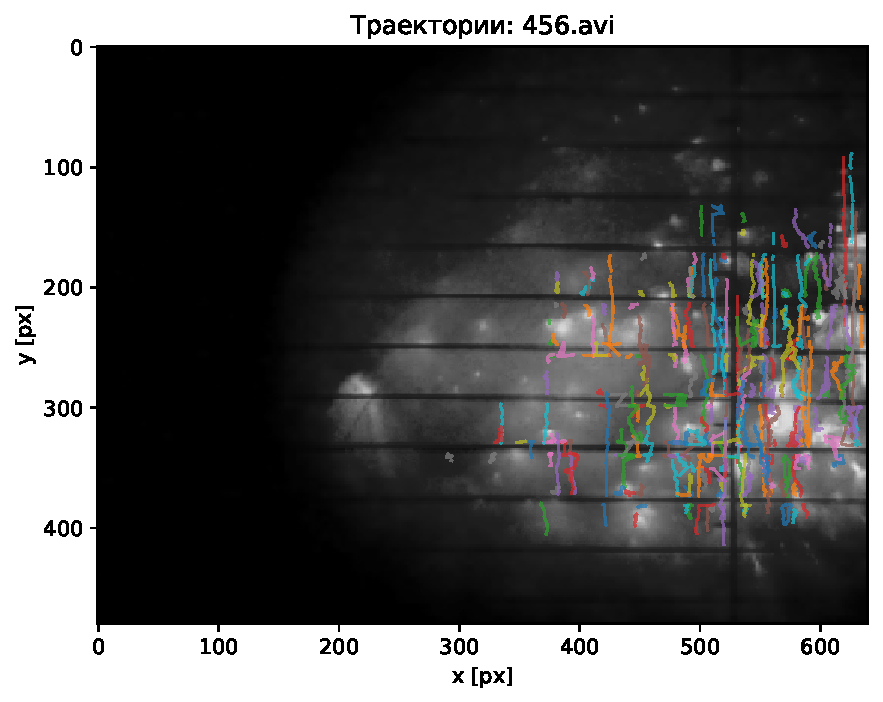
\includegraphics[width=\textwidth]{456_1_trajectories.pdf}
    \end{subfigure}
    \hfill
    \begin{subfigure}[b]{0.32\textwidth}
        \centering
        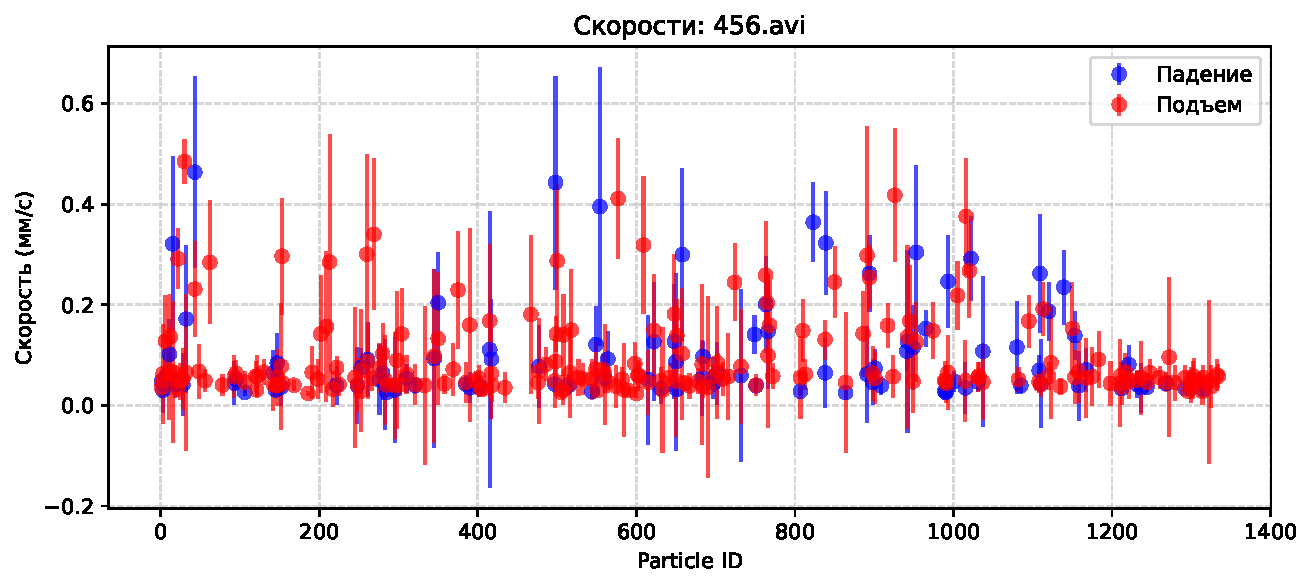
\includegraphics[width=\textwidth]{456_2_speeds.pdf}
    \end{subfigure}
    \hfill
    \begin{subfigure}[b]{0.32\textwidth}
        \centering
        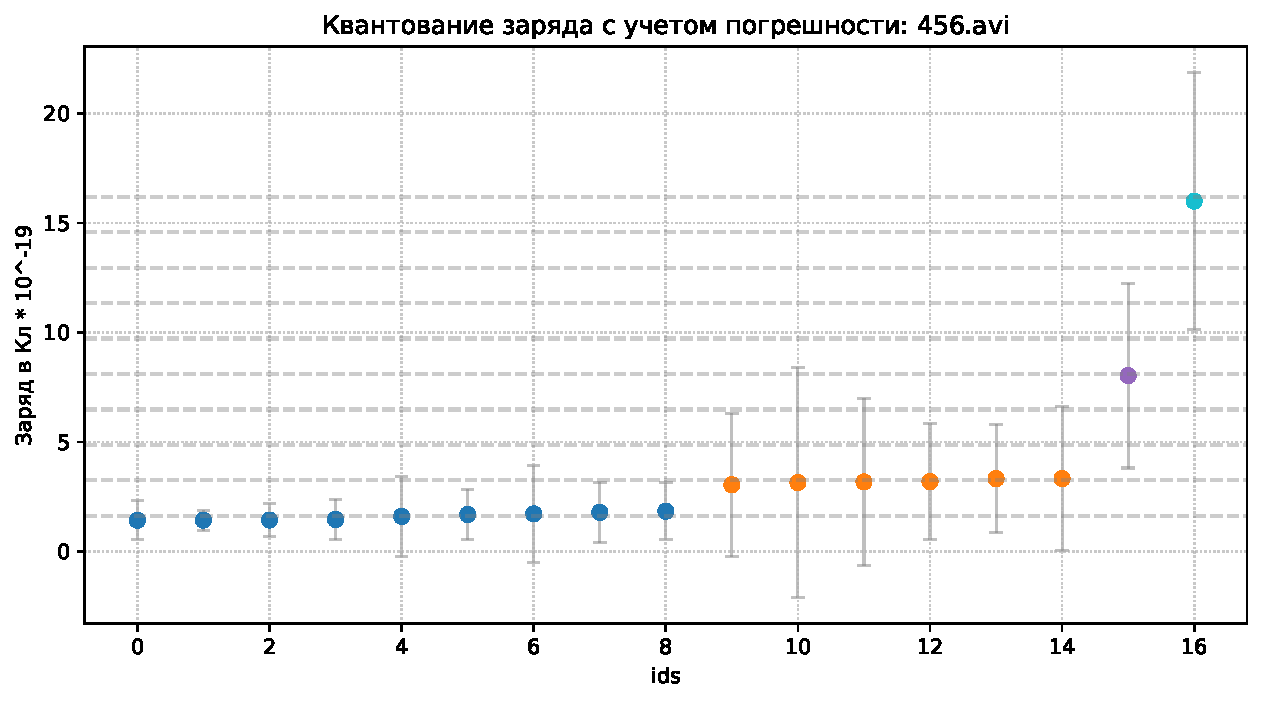
\includegraphics[width=\textwidth]{456_3_quantization.pdf}
    \end{subfigure}
    \caption{Результаты обработки серии \texttt{456}.}
\end{figure*}

% --- Серия 2323-0195_10X ---
\begin{figure*}[htbp]
    \centering
    \begin{subfigure}[b]{0.32\textwidth}
        \centering
        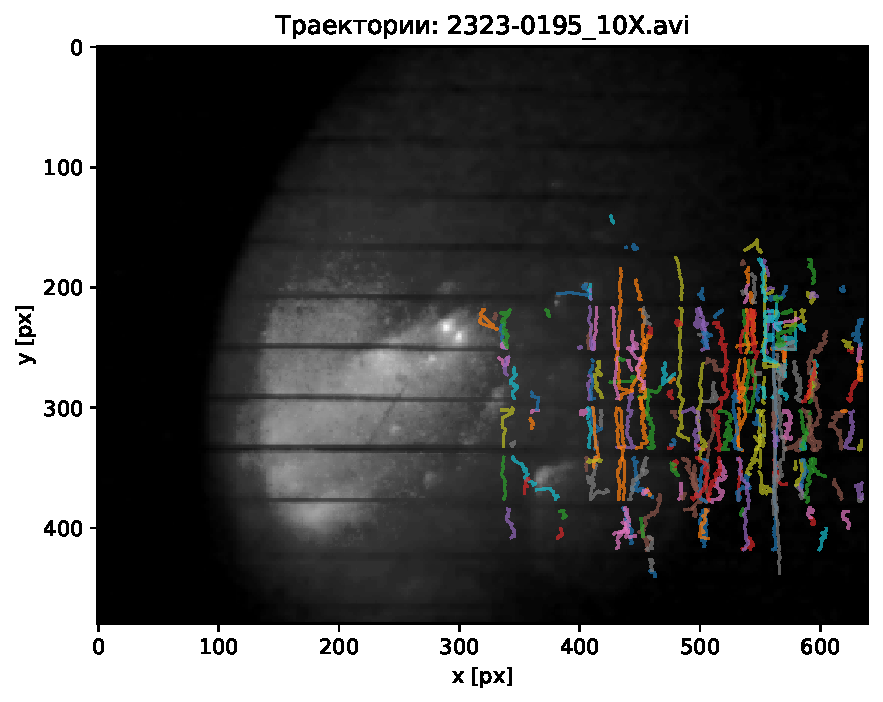
\includegraphics[width=\textwidth]{2323-0195_10X_1_trajectories.pdf}
    \end{subfigure}
    \hfill
    \begin{subfigure}[b]{0.32\textwidth}
        \centering
        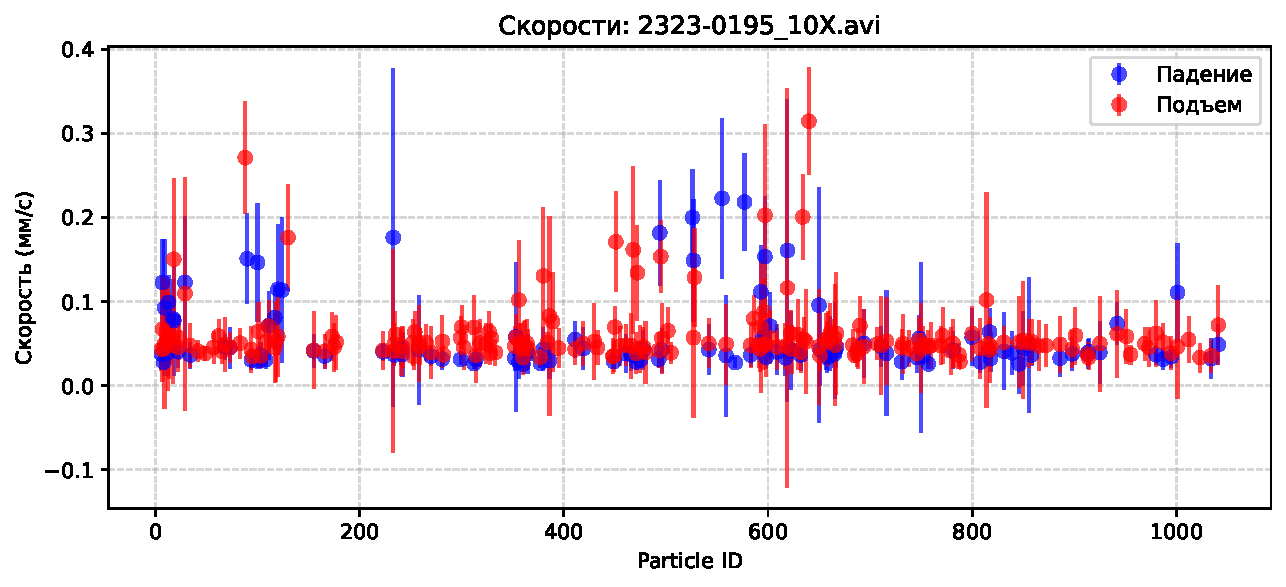
\includegraphics[width=\textwidth]{2323-0195_10X_2_speeds.pdf}
    \end{subfigure}
    \hfill
    \begin{subfigure}[b]{0.32\textwidth}
        \centering
        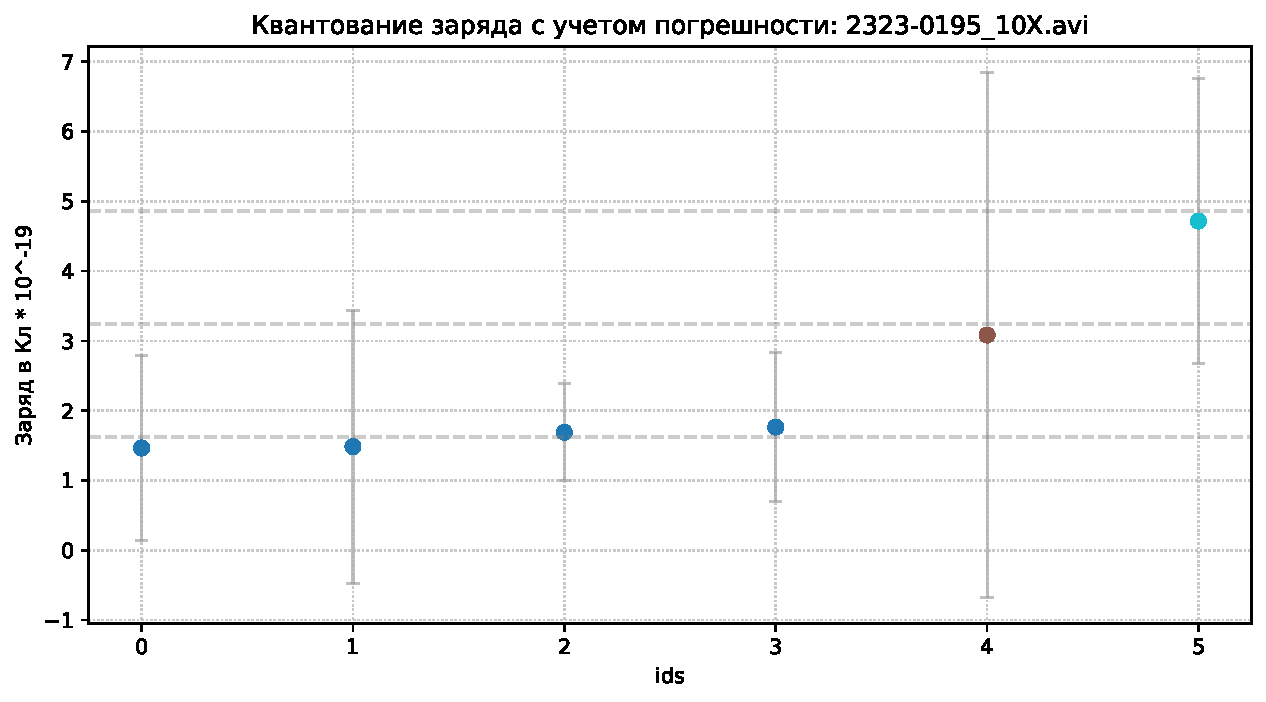
\includegraphics[width=\textwidth]{2323-0195_10X_3_quantization.pdf}
    \end{subfigure}
    \caption{Результаты обработки серии \texttt{2323-0195\_10X}.}
\end{figure*}

% --- Серия 87970 ---
\begin{figure*}[htbp]
    \centering
    \begin{subfigure}[b]{0.32\textwidth}
        \centering
        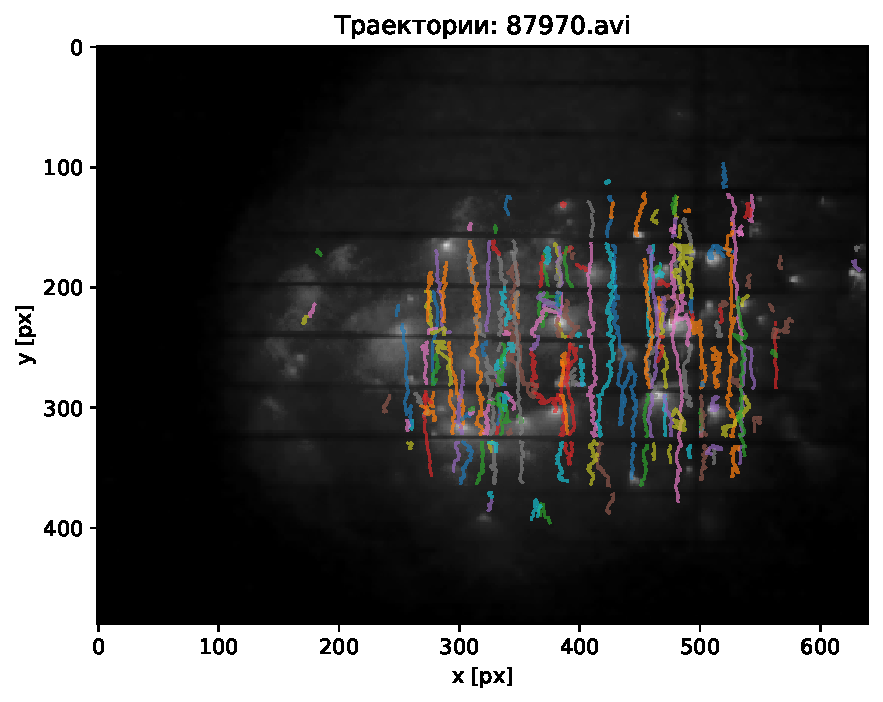
\includegraphics[width=\textwidth]{87970_1_trajectories.pdf}
    \end{subfigure}
    \hfill
    \begin{subfigure}[b]{0.32\textwidth}
        \centering
        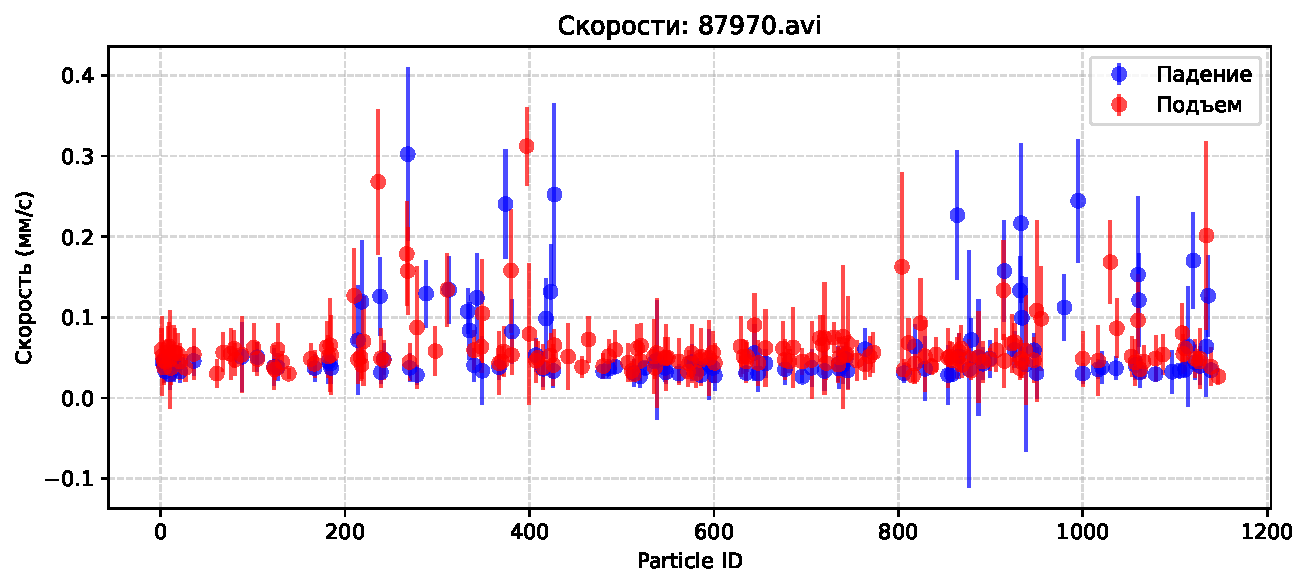
\includegraphics[width=\textwidth]{87970_2_speeds.pdf}
    \end{subfigure}
    \hfill
    \begin{subfigure}[b]{0.32\textwidth}
        \centering
        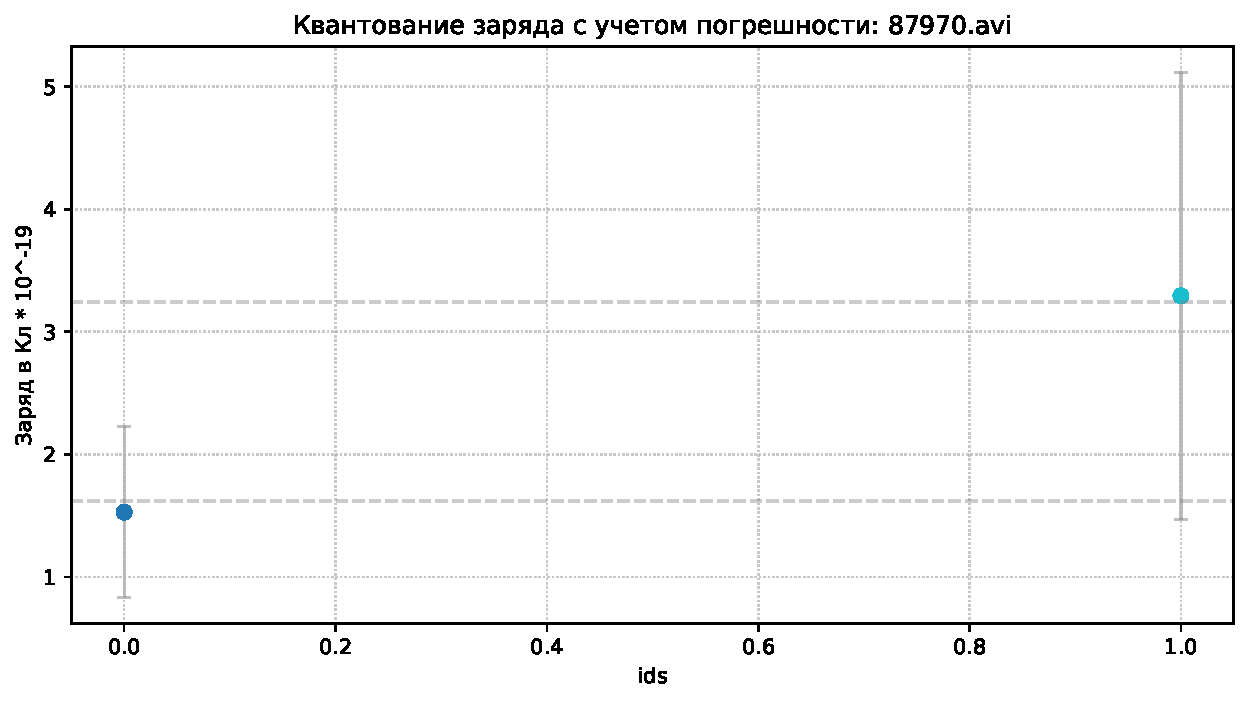
\includegraphics[width=\textwidth]{87970_3_quantization.pdf}
    \end{subfigure}
    \caption{Результаты обработки серии \texttt{87970}.}
\end{figure*}

% --- Серия 098098 ---
\begin{figure*}[htbp]
    \centering
    \begin{subfigure}[b]{0.32\textwidth}
        \centering
        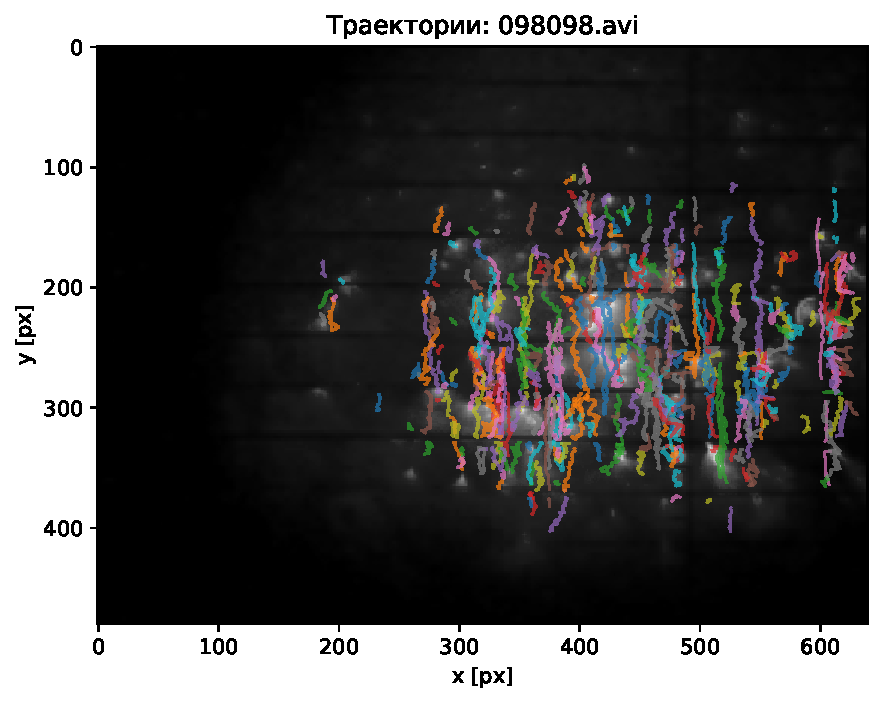
\includegraphics[width=\textwidth]{098098_1_trajectories.pdf}
    \end{subfigure}
    \hfill
    \begin{subfigure}[b]{0.32\textwidth}
        \centering
        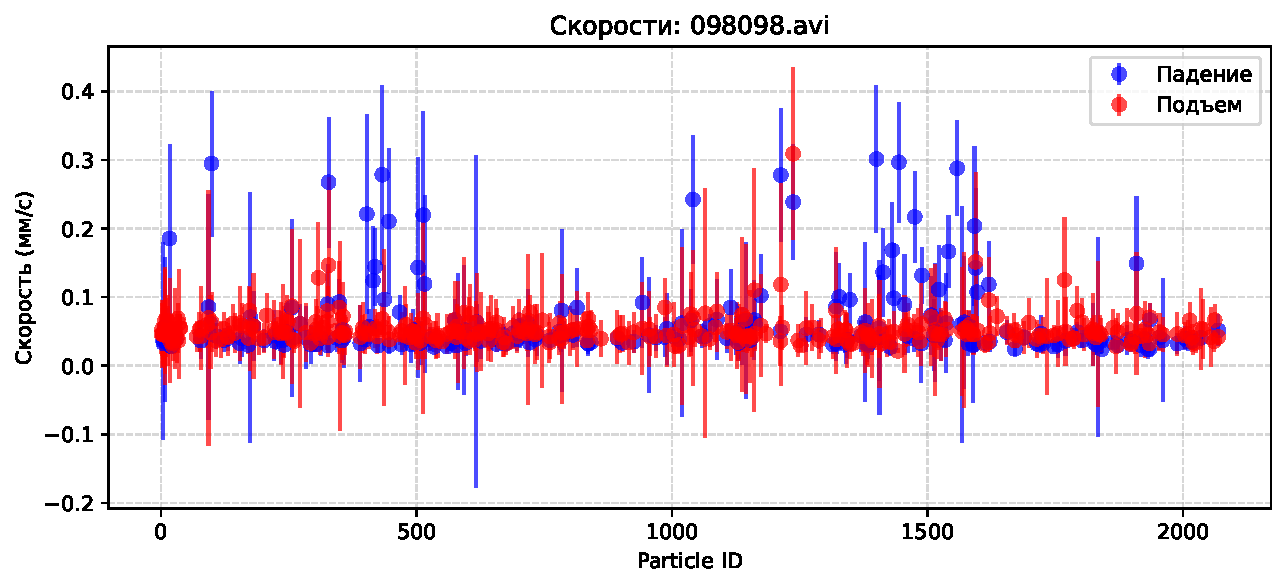
\includegraphics[width=\textwidth]{098098_2_speeds.pdf}
    \end{subfigure}
    \hfill
    \begin{subfigure}[b]{0.32\textwidth}
        \centering
        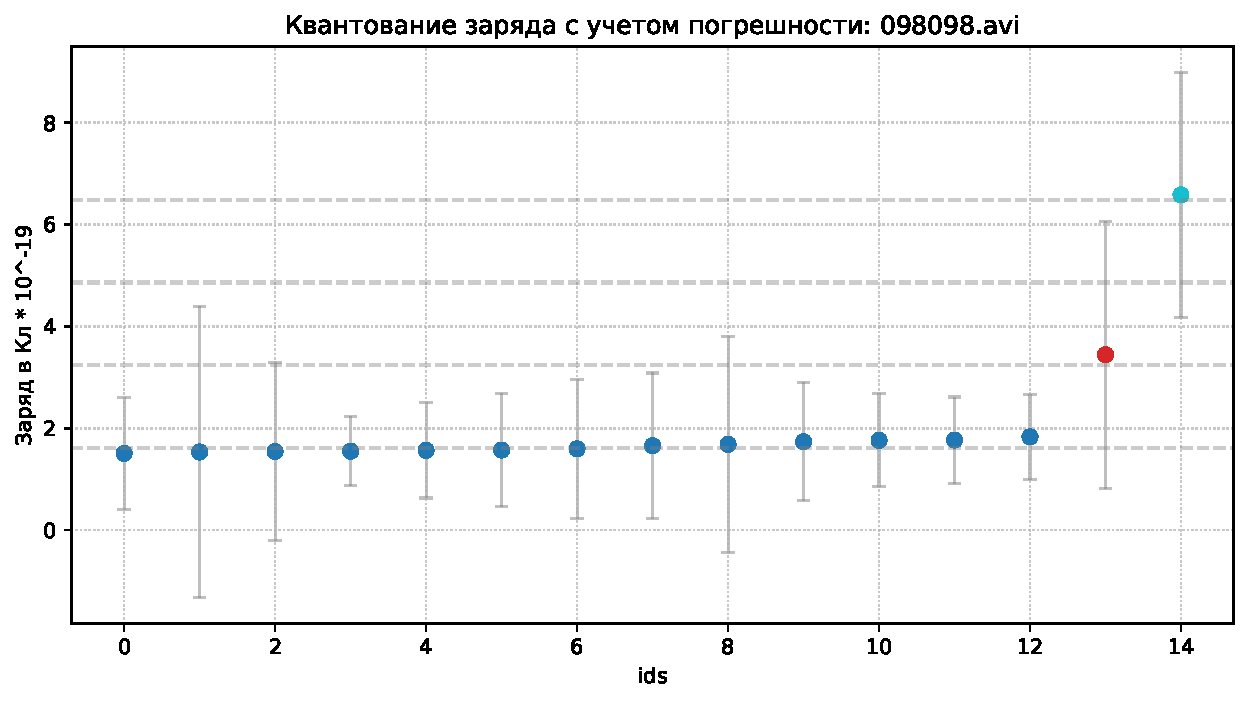
\includegraphics[width=\textwidth]{098098_3_quantization.pdf}
    \end{subfigure}
    \caption{Результаты обработки серии \texttt{098098}.}
\end{figure*}

% --- Серия l567X ---
\begin{figure*}[htbp]
    \centering
    \begin{subfigure}[b]{0.32\textwidth}
        \centering
        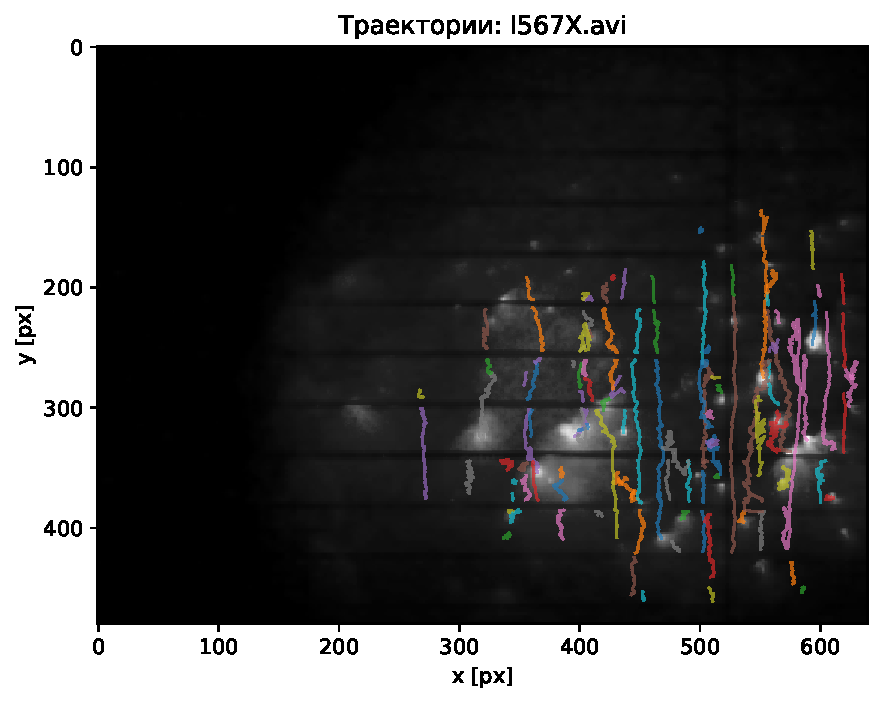
\includegraphics[width=\textwidth]{I567X_1_trajectories.pdf}
    \end{subfigure}
    \hfill
    \begin{subfigure}[b]{0.32\textwidth}
        \centering
        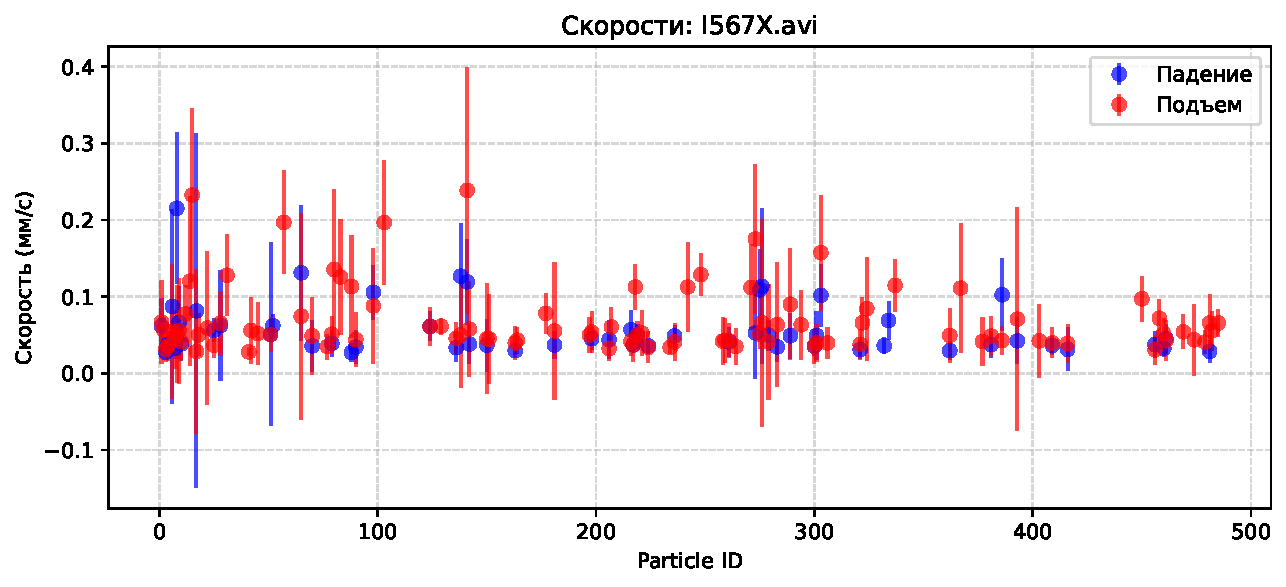
\includegraphics[width=\textwidth]{I567X_2_speeds.pdf}
    \end{subfigure}
    \hfill
    \begin{subfigure}[b]{0.32\textwidth}
        \centering
        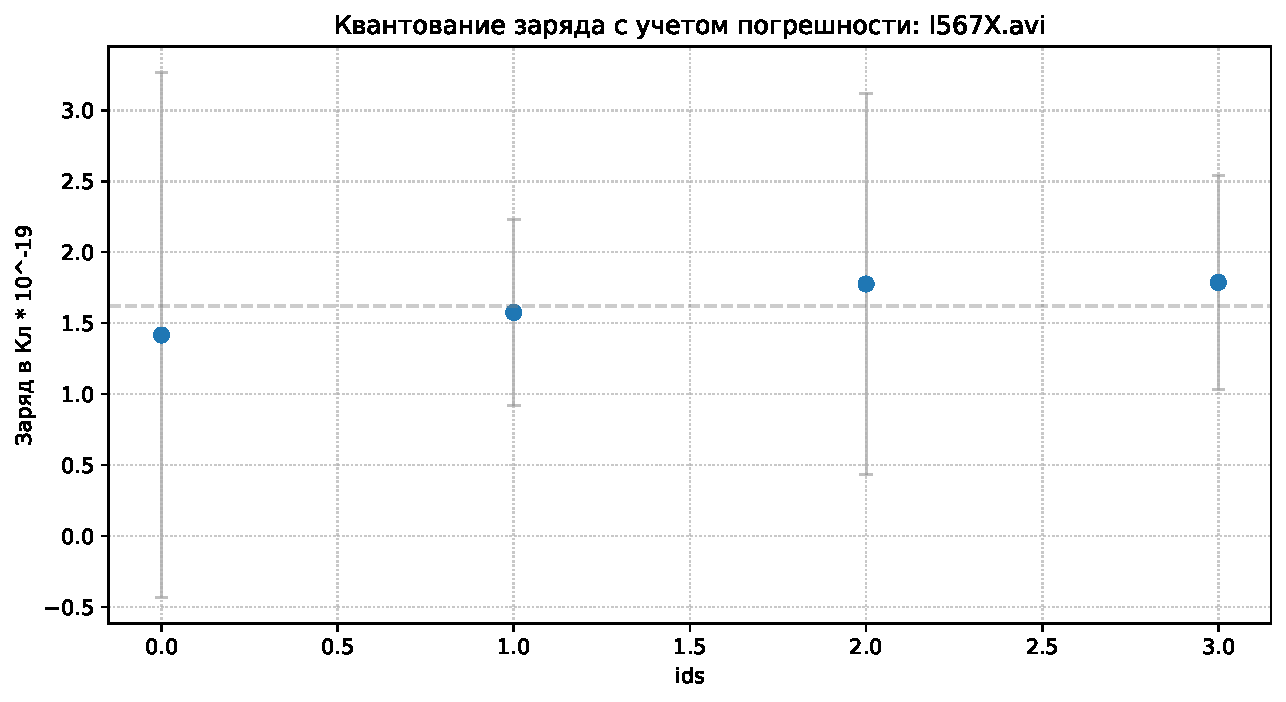
\includegraphics[width=\textwidth]{I567X_3_quantization.pdf}
    \end{subfigure}
    \caption{Результаты обработки серии \texttt{l567X}.}
\end{figure*}

% --- Серия l56756 ---
\begin{figure*}[htbp]
    \centering
    \begin{subfigure}[b]{0.32\textwidth}
        \centering
        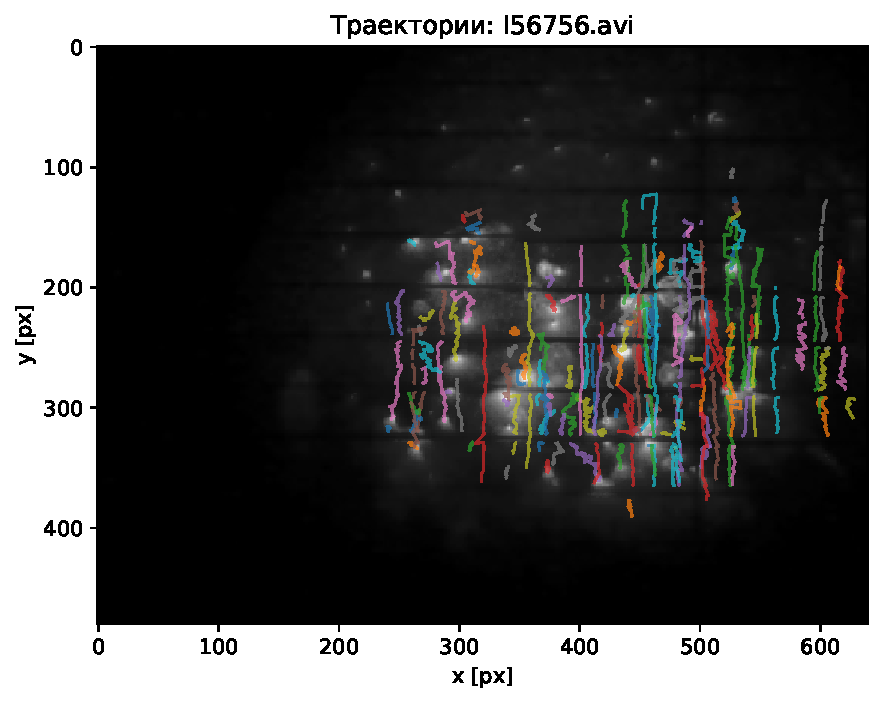
\includegraphics[width=\textwidth]{I56756_1_trajectories.pdf}
    \end{subfigure}
    \hfill
    \begin{subfigure}[b]{0.32\textwidth}
        \centering
        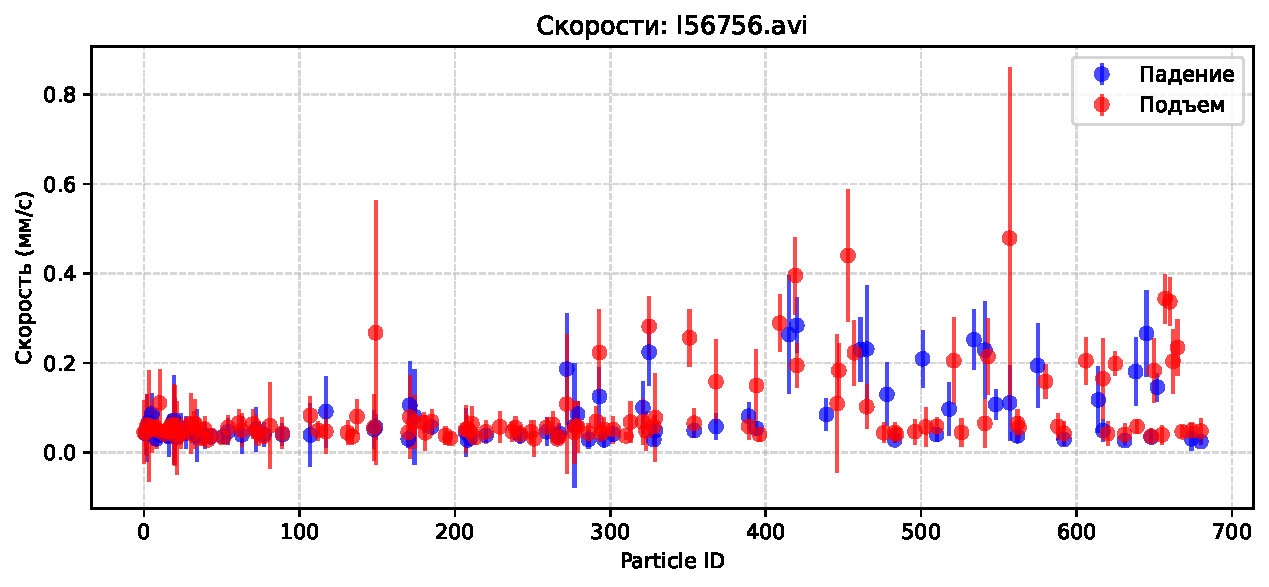
\includegraphics[width=\textwidth]{I56756_2_speeds.pdf}
    \end{subfigure}
    \hfill
    \begin{subfigure}[b]{0.32\textwidth}
        \centering
        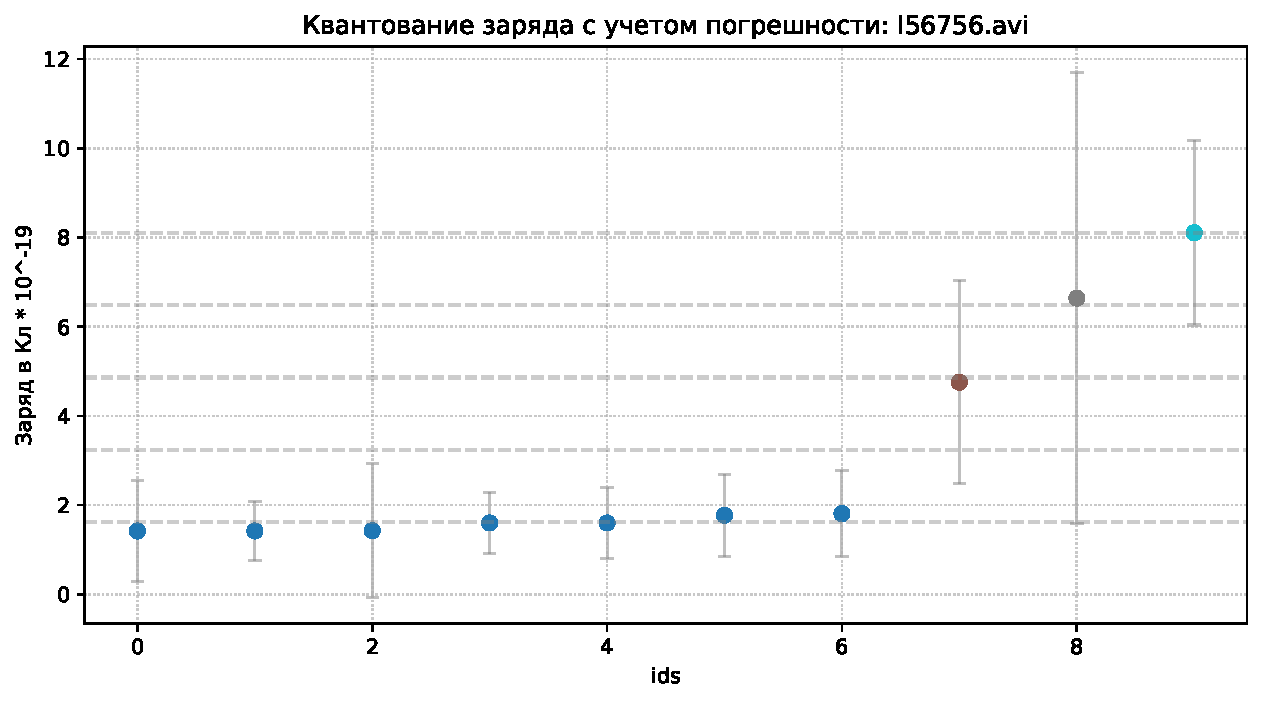
\includegraphics[width=\textwidth]{I56756_3_quantization.pdf}
    \end{subfigure}
    \caption{Результаты обработки серии \texttt{l56756}.}
\end{figure*}

% --- Серия IMG.jpg-0184_10X ---
\begin{figure*}[htbp]
    \centering
    \begin{subfigure}[b]{0.32\textwidth}
        \centering
        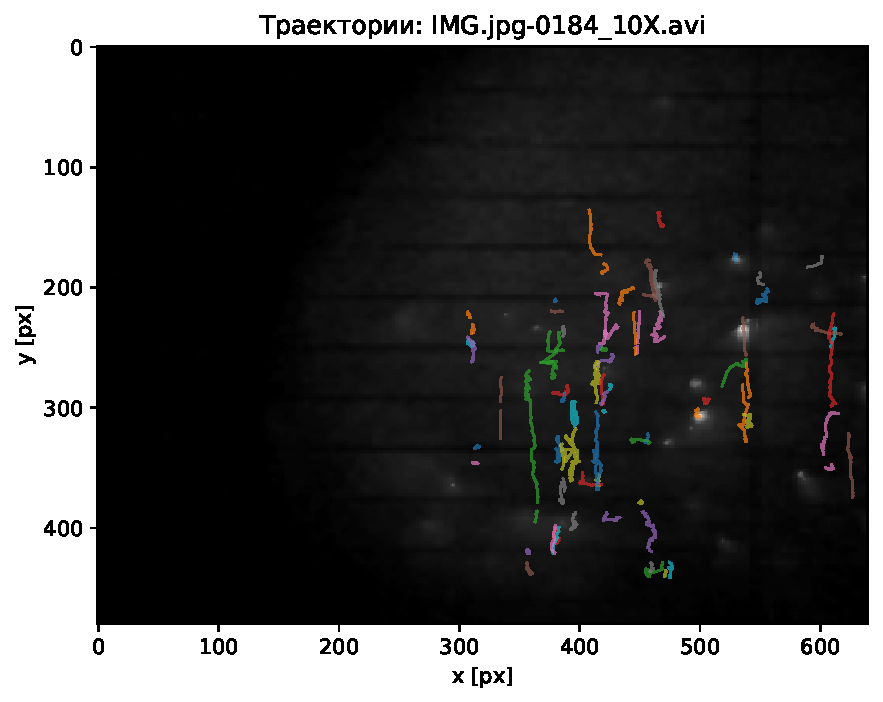
\includegraphics[width=\textwidth]{IMG.jpg-0184_10X_1_trajectories.pdf}
    \end{subfigure}
    \hfill
    \begin{subfigure}[b]{0.32\textwidth}
        \centering
        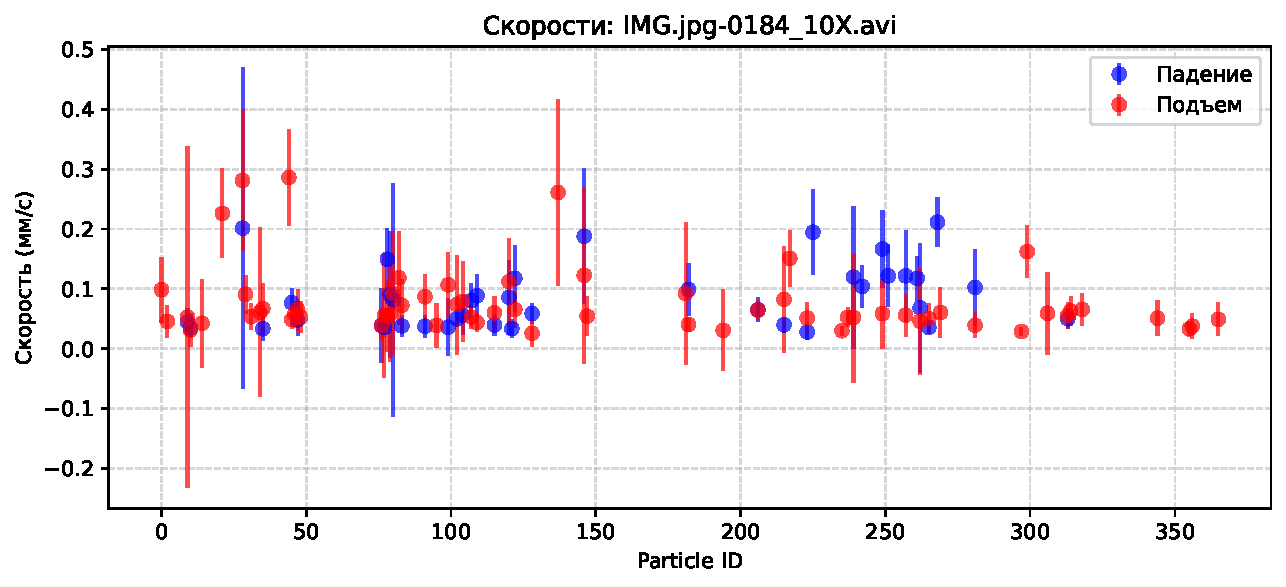
\includegraphics[width=\textwidth]{IMG.jpg-0184_10X_2_speeds.pdf}
    \end{subfigure}
    \hfill
    \begin{subfigure}[b]{0.32\textwidth}
        \centering
        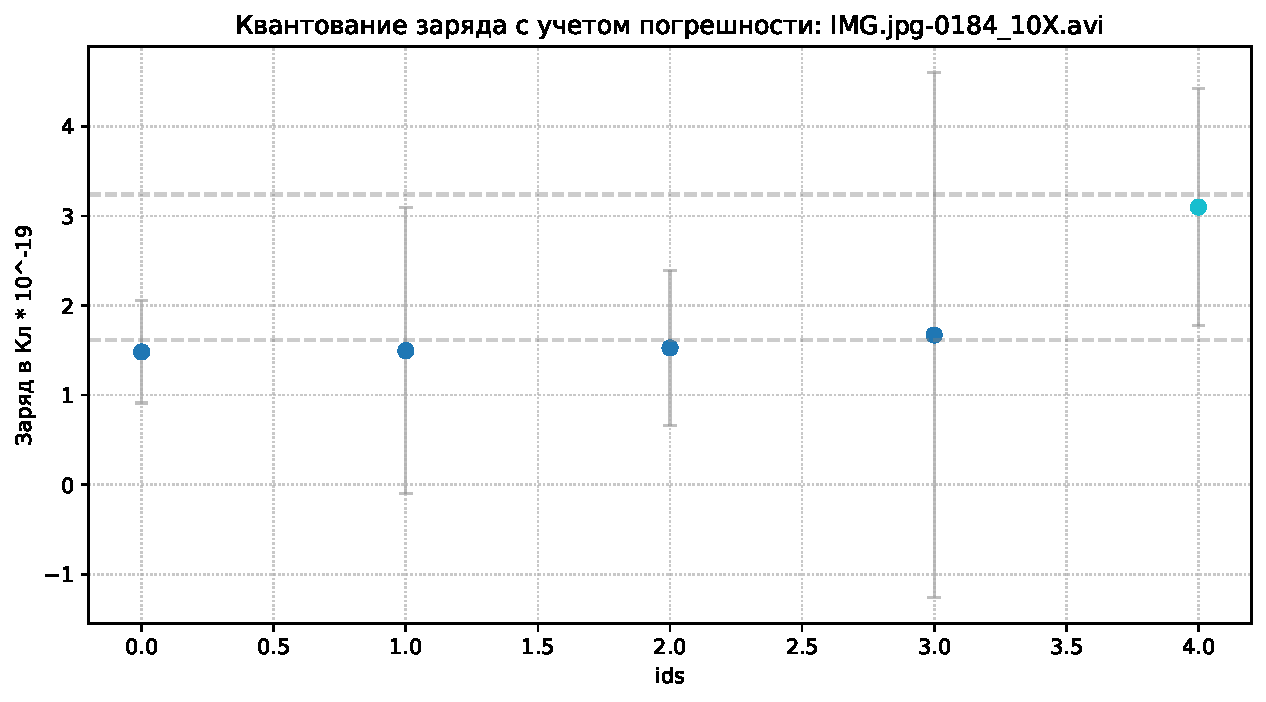
\includegraphics[width=\textwidth]{IMG.jpg-0184_10X_3_quantization.pdf}
    \end{subfigure}
    \caption{Результаты обработки серии \texttt{IMG.jpg-0184\_10X}.}
\end{figure*}

% --- Серия test ---
\begin{figure*}[htbp]
    \centering
    \begin{subfigure}[b]{0.32\textwidth}
        \centering
        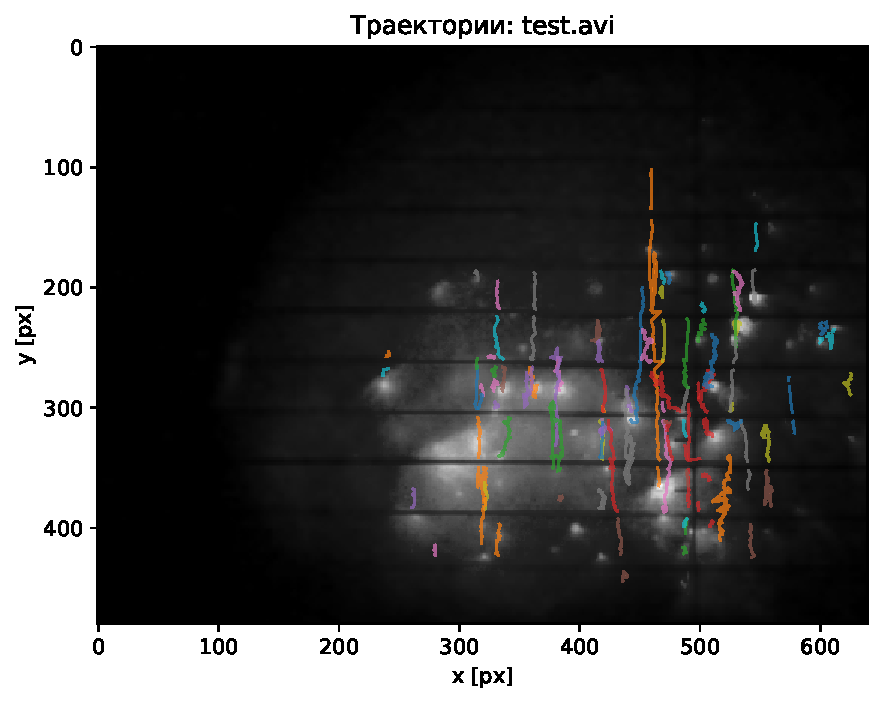
\includegraphics[width=\textwidth]{test_1_trajectories.pdf}
    \end{subfigure}
    \hfill
    \begin{subfigure}[b]{0.32\textwidth}
        \centering
        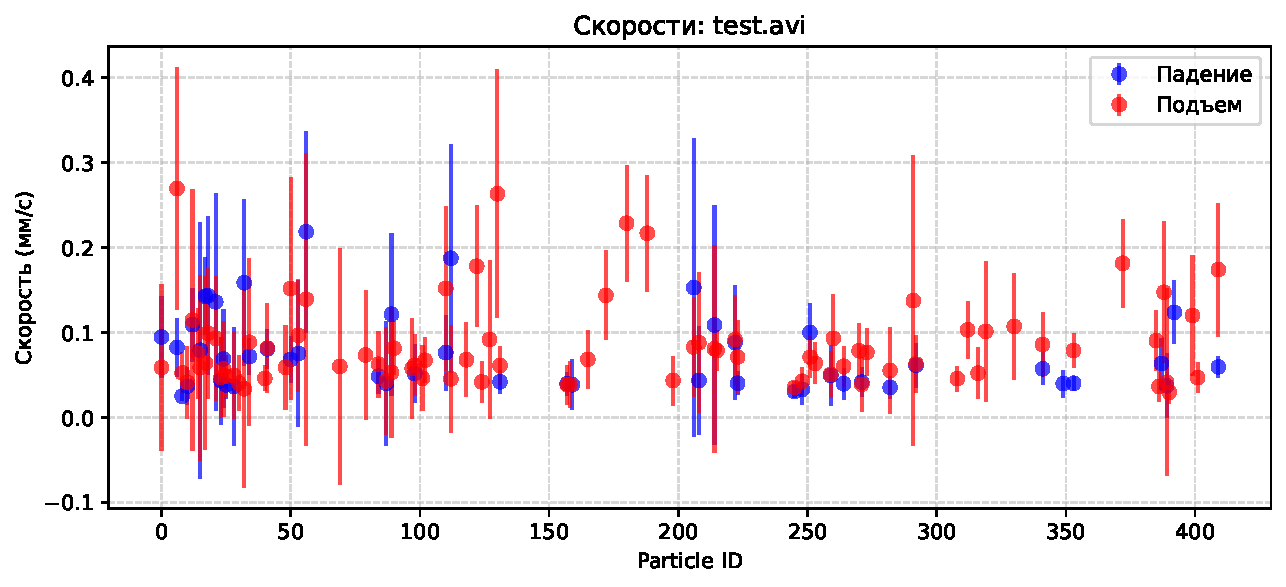
\includegraphics[width=\textwidth]{test_2_speeds.pdf}
    \end{subfigure}
    \hfill
    \begin{subfigure}[b]{0.32\textwidth}
        \centering
        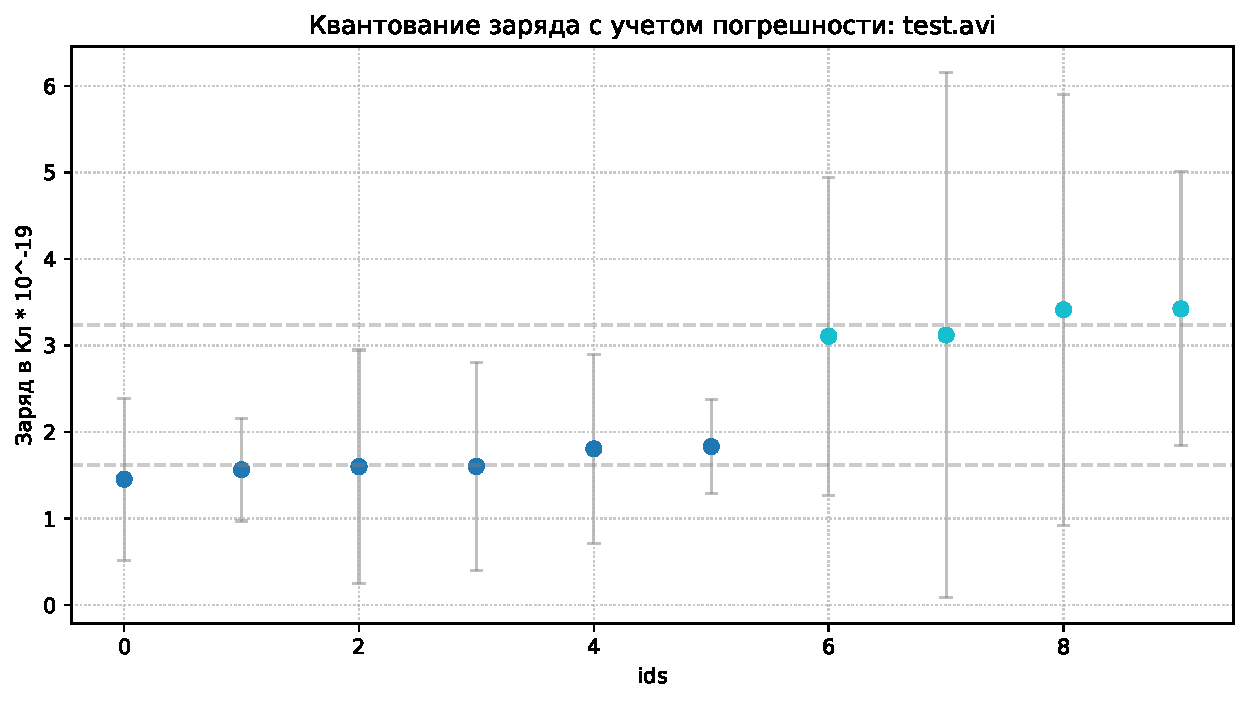
\includegraphics[width=\textwidth]{test_3_quantization.pdf}
    \end{subfigure}
    \caption{Результаты обработки серии \texttt{test}.}
\end{figure*}


% --- Библиография ---
\begin{thebibliography}{99}
\bibitem{practicum2019}
Никулин М. Г., Попов П. В. и др. \textit{Лабораторный практикум по общей физике. Том 2. Электричество и магнетизм.} — М.: МФТИ, 2019.
\end{thebibliography}

\end{document}